\chapter{Representación Gráfica del Movimiento Unidimensional}
\section{Graficos Posicion Tiempo}

\subsection{a) Gráfica de posición vs tiempo}
\begin{center}
    \begin{tikzpicture}[scale=1]
        % Ejes
        \draw[->] (0,0) -- (4,0) node[right] {$t$};
        \draw[->] (0,0) -- (0,4) node[above] {$x$};
        
        % Curva
        \draw[thick] (0.5,1) .. controls (1.5,2.8) and (2.5,2.5) .. (3.5,3.5);
        
        % Puntos y líneas auxiliares
        \draw[dashed] (1,1.7) -- (1,0) node[below] {$t_0$};
        \draw[dashed] (3,3) -- (3,0) node[below] {$t$};
        \draw[dashed] (1,1.7) -- (0,1.7) node[left] {$x(t_0)$};
        \draw[dashed] (3,3) -- (0,3) node[left] {$x(t)$};
    \end{tikzpicture}
\end{center}

\subsection{b) Velocidad media}
\begin{center}
    \begin{tikzpicture}[scale=1]
        % Ejes
        \draw[->] (0,0) -- (4,0) node[right] {$t$};
        \draw[->] (0,0) -- (0,4) node[above] {$x$};
        
        % Curva
        \draw[thick] (0.5,1) .. controls (1.5,2.8) and (2.5,2.5) .. (3.5,3.5);
        
        % Puntos y líneas auxiliares
        \draw[dashed] (1,1.5) -- (1,0) node[below] {$t_1$};
        \draw[dashed] (3,3) -- (3,0) node[below] {$t_2$};
        \draw[dashed] (1,1.5) -- (0,1.5) node[left] {$x_1$};
        \draw[dashed] (3,3) -- (0,3) node[left] {$x_2$};
        
        % Línea de velocidad media
        \draw[thick] (1,1.5) -- (3,3);
    \end{tikzpicture}
\end{center}

\subsection{c) Velocidad instantánea}
\begin{center}
    \begin{tikzpicture}[scale=1]
        % Ejes
        \draw[->] (0,0) -- (4,0) node[right] {$t$};
        \draw[->] (0,0) -- (0,4) node[above] {$x$};
        
        % Curva
        \draw[thick] (0.5,1) .. controls (1.5,2.8) and (2.5,2.5) .. (3.5,3.5);
        
        % Punto y tangente
        \draw[dashed] (2,2.5) -- (2,0) node[below] {$t$};
        \draw[dashed] (2,2.5) -- (0,2.5) node[left] {$x$};
        \draw[thick] (1,2) -- (3,3);
    \end{tikzpicture}
\end{center}

\subsection{Fórmulas}
\begin{align}
    V_{\text{med}} &= \frac{x_2 - x_1}{t_2 - t_1} = \frac{\Delta x}{\Delta t} \\
    V &= \lim_{\Delta t \to 0} \frac{\Delta x}{\Delta t} = \frac{dx}{dt}
\end{align}
La velocidad en un gráfico posición vs tiempo representa la pendiente de la recta tangente a la curva.
\subsection{d) Aceleración (signo)}
\begin{center}
    \begin{tikzpicture}[scale=1]
        % Ejes
        \draw[->] (-1,0) -- (4,0) node[right] {$t$};
        \draw[->] (0,-1) -- (0,4) node[above] {$x$};
        
        % Curva
        \draw[thick] (0.5,0.5) .. controls (1.5,2) and (2.5,3) .. (3.5,3.8);
        
        % Texto
        \node at (3,2) {$a < 0$};
    \end{tikzpicture}
\end{center}
\begin{align}
    a &= \frac{dv}{dt} = \frac{d}{dt} \left( \frac{dx}{dt} \right) \\
    a &= \frac{d^2x}{dt^2}
\end{align}

\begin{center}
    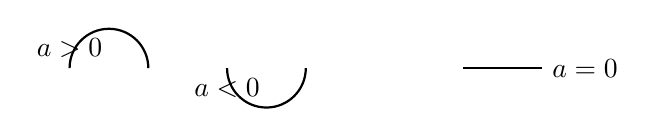
\begin{tikzpicture}
        \draw[thick] (0,0) arc (0:180:0.5) node[above] {$a > 0$};
        \draw[thick] (2,0) arc (0:-180:0.5) node[below] {$a < 0$};
        \draw[thick] (4,0) -- (5,0) node[right] {$a = 0$};
    \end{tikzpicture}
\end{center}
La aceleración es la derivada de la velocidad con respecto al tiempo, y su signo indica la curvatura de la gráfica de posición.

\newpage
\section{Graficos Velocidad Tiempo}
\subsection{(a) La Velocidad en cualquier instante}

\begin{center}
\begin{tikzpicture}[scale=1]
    % Ejes
    \draw[->] (0,0) -- (4,0) node[right] {$t$};
    \draw[->] (0,0) -- (0,4) node[above] {$V$};
    
    % Curva
    \draw[thick] (0.5,1) .. controls (1.5,1.8) .. (3.5,3.5) node[right] {$V(t)$};
    
    % Líneas de referencia
    \draw[dashed] (1.8,2.2) -- (1.8,0) node[below] {$t$};
    \draw[dashed] (1.8,2.2) -- (0,2.2);
\end{tikzpicture}
\end{center}

\subsection{(b) Aceleración media}

La aceleración media está dada por:
\[
A_{\text{med}} = \frac{\Delta V}{\Delta t} = \frac{V_2 - V_1}{t_2 - t_1}
\]

\begin{center}
\begin{tikzpicture}[scale=1]
    % Ejes
    \draw[->] (0,0) -- (4,0) node[right] {$t$};
    \draw[->] (0,0) -- (0,4) node[above] {$V$};
    
    % Curva
    \draw[thick] (0.5,1) .. controls (1.5,1.8) .. (3.5,3.5);
    
    % Líneas de referencia
    \draw[dashed] (1,1.5) -- (1,0) node[below] {$t_1$};
    \draw[dashed] (3,3) -- (3,0) node[below] {$t_2$};
    \draw[dashed] (1,1.5) -- (0,1.5) node[left] {$V_1$};
    \draw[dashed] (3,3) -- (0,3) node[left] {$V_2$};
    
    % Recta tangente
    \draw[thick] (0.8,1.3) -- (3.2,3.2);
    \end{tikzpicture}
    \end{center}

\subsection{(c) Aceleración}
\[
a = \lim_{\Delta t \to 0} \frac{\Delta v}{\Delta t} = \frac{dv}{dt}
\]

\subsection{(d) Desplazamiento}
\[
V = \frac{dx}{dt}
\]
\[
dx = V \, dt
\]
\[
\int_{t_1}^{t_2} dx = \int_{t_1}^{t_2} V \, dt
\]
\[
x(t_2) - x(t_1) = \int_{t_1}^{t_2} V \, dt
\]

\subsection{Gráficos}

\begin{center}
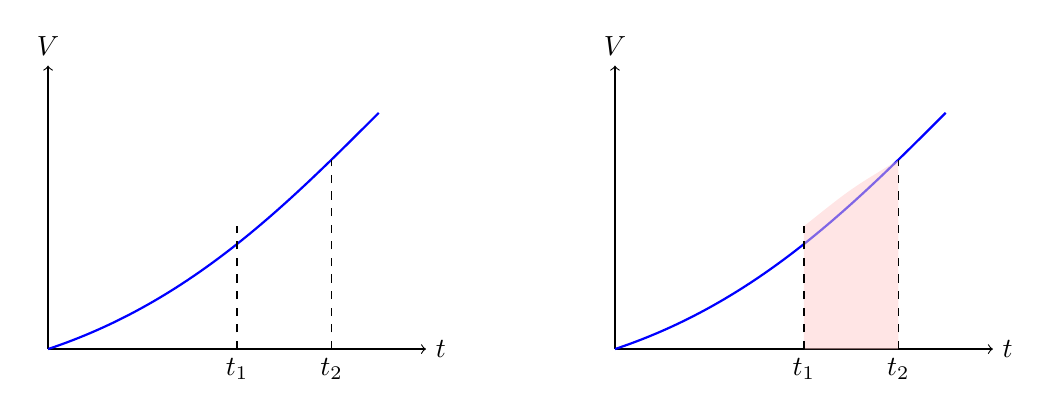
\begin{tikzpicture}[scale=1.2]
  % Primer gráfico
  \draw[->] (0, 0) -- (4, 0) node[right] {$t$};
  \draw[->] (0, 0) -- (0, 3) node[above] {$V$};
  \draw[thick, blue] (0, 0) .. controls (1.5, 0.5) and (2.5, 1.5) .. (3.5, 2.5);
  \draw[dashed] (2, 0) -- (2, 1.3) node[above right] {};
  \draw[dashed] (3, 0) -- (3, 2) node[above right] {};
  \node[below] at (2, 0) {$t_1$};
  \node[below] at (3, 0) {$t_2$};

  % Segundo gráfico
  \begin{scope}[xshift=6cm]
    \draw[->] (0, 0) -- (4, 0) node[right] {$t$};
    \draw[->] (0, 0) -- (0, 3) node[above] {$V$};
    \draw[thick, blue] (0, 0) .. controls (1.5, 0.5) and (2.5, 1.5) .. (3.5, 2.5);
    \fill[red!20, opacity=0.5] (2, 0) -- (2, 1.3) .. controls (2.5, 1.7) .. (3, 2) -- (3, 0) -- cycle;
    \draw[dashed] (2, 0) -- (2, 1.3);
    \draw[dashed] (3, 0) -- (3, 2);
    \node[below] at (2, 0) {$t_1$};
    \node[below] at (3, 0) {$t_2$};
  \end{scope}
\end{tikzpicture}
\end{center}

\[
\text{Área bajo la curva en el gráfico } V \text{ vs tiempo.}
\]

\newpage
\section{Graficos Aceleración Tiempo}

Información que nos entrega:  
\emph{La aceleración en cualquier instante de tiempo.}

\begin{center}
\begin{tikzpicture}[scale=1.2]
  % Ejes
  \draw[->] (0, 0) -- (5, 0) node[right] {$t$};
  \draw[->] (0, 0) -- (0, 3) node[above] {$a$};

  % Curva
  \draw[thick] (0, 0) .. controls (2, 0.5) and (3, 1.5) .. (4, 2.5);

  % Punto en la curva
  \filldraw (2.8, 1.3) circle (2pt) node[right] {$a(t)$};

  % Líneas punteadas
  \draw[dashed] (2.8, 0) -- (2.8, 1.3);
  \draw[dashed] (0, 1.3) -- (2.8, 1.3);

  % Etiquetas de los puntos
  \node[below] at (2.8, 0) {$t$};
  \node[left] at (0, 1.3) {$a(t)$};
\end{tikzpicture}
\end{center}

\newpage
\section{Casos Particulares}
\subsection{Movimiento Rectilíneo Uniforme (M.R.U.)}

\textbf{Posición vs tiempo:}
\[
x(t) = x_0 + vt
\]

\begin{center}
\begin{tikzpicture}[scale=1.2]
  % Ejes
  \draw[->] (0, 0) -- (4, 0) node[right] {$t$};
  \draw[->] (0, 0) -- (0, 3) node[above] {$x$};

  % Línea recta
  \draw[thick] (0, 1) -- (3.5, 2.5) node[right] {};
  \node[left] at (0, 1) {$x_0$};
\end{tikzpicture}
\end{center}

\textbf{Velocidad vs tiempo:}
\[
v = \text{cte}
\]

\begin{center}
\begin{tikzpicture}[scale=1.2]
  % Ejes
  \draw[->] (0, 0) -- (4, 0) node[right] {$t$};
  \draw[->] (0, 0) -- (0, 2) node[above] {$v$};

  % Línea constante
  \draw[thick] (0, 1) -- (3.5, 1);
  \node[left] at (0, 1) {$v$};
\end{tikzpicture}
\end{center}

\subsection{Movimiento Rectilíneo Uniformemente Acelerado (M.R.U.A.)}

\textbf{Posición vs tiempo:}
\[
x(t) = x_0 + v_0 t + \frac{1}{2} a t^2
\]

\begin{center}
\begin{tikzpicture}[scale=1.2]
  % Ejes
  \draw[->] (0, 0) -- (4, 0) node[right] {$t$};
  \draw[->] (0, 0) -- (0, 3) node[above] {$x$};

  % Curva cuadrática
  \draw[thick] (0, 0) parabola (3, 2.5);
\end{tikzpicture}
\end{center}

\textbf{Velocidad vs tiempo:}
\[
v(t) = v_0 + at
\]

\begin{center}
\begin{tikzpicture}[scale=1.2]
  % Ejes
  \draw[->] (0, 0) -- (4, 0) node[right] {$t$};
  \draw[->] (0, 0) -- (0, 3) node[above] {$v$};

  % Línea recta
  \draw[thick] (0, 1) -- (3, 2.5);
  \node[left] at (0, 1) {$v_0$};
\end{tikzpicture}
\end{center}

\textbf{Aceleración vs tiempo:}
\[
a = \text{cte}
\]

\begin{center}
\begin{tikzpicture}[scale=1.2]
  % Ejes
  \draw[->] (0, 0) -- (4, 0) node[right] {$t$};
  \draw[->] (0, 0) -- (0, 2) node[above] {$a$};

  % Línea constante
  \draw[thick] (0, 1) -- (3.5, 1);
  \node[left] at (0, 1) {$a$};
\end{tikzpicture}
\end{center}

\subsection{Ejemplo: Lanzamiento vertical hacia arriba}

\textbf{Velocidad vs tiempo:}

\begin{center}
\begin{tikzpicture}[scale=1.2]
  % Ejes
  \draw[->] (0, 0) -- (4, 0) node[right] {$t$};
  \draw[->] (0, -2) -- (0, 2.5) node[above] {$v$};

  % Línea descendente
  \draw[thick] (0, 2) -- (3, -2);
  \node[left] at (0, 2) {$v_0$};
  \node[below] at (3, -2) {$t$};
\end{tikzpicture}
\end{center}

\textbf{Posición vs tiempo:}

\begin{center}
\begin{tikzpicture}[scale=1.2]
  % Ejes
  \draw[->] (0, 0) -- (4, 0) node[right] {$t$};
  \draw[->] (0, 0) -- (0, 3) node[above] {$x$};

  % Curva parabólica
  \draw[thick] (0, 0) parabola bend (2, 2.5) (3, 0);
  \node[below] at (3, 0) {$t$};
\end{tikzpicture}
\end{center}

\noindent
\textbf{Ej:} La posición de un móvil se muestra en la fig. El móvil se mueve unidimensionalmente.

\vspace{0.3cm}

\noindent
\textbf{Del $\Rightarrow$}

\begin{enumerate}
    \item[a)] La posición en los instantes: $T=0$, $T=3$, $T=6$, $T=12$.
    \item[b)] El desplazamiento entre:
    \begin{itemize}
        \item $T=0$ y $T=3$ s
        \item $T=0$ y $T=6$ s
        \item $T=6$ y $T=12$ s
    \end{itemize}
    \item[c)] La velocidad media entre:
    \begin{itemize}
        \item $T=0$ y $T=3$ s
        \item $T=0$ y $T=6$ s
        \item $T=6$ y $T=12$ s
    \end{itemize}
    \item[d)] Hago el gráfico de velocidad vs tiempo para el móvil.
\end{enumerate}

\vspace{0.3cm}
\noindent
\textbf{Gráfico:}

\begin{center}
\begin{tikzpicture}[scale=0.8]
    % Ejes
    \draw[->] (0,0) -- (6,0) node[right] {$t$ (s)};
    \draw[->] (0,-2) -- (0,4) node[above] {$X(t)$ (m)};

    % Líneas de referencia
    \draw[dashed] (2,0) -- (2,3);
    \draw[dashed] (4,0) -- (4,1);

    % Curva de posición
    \draw[thick] (0,-1) -- (2,3) -- (4,1) -- (6,0);

    % Etiquetas
    \node at (-0.3,-1) {$-10$};
    \node at (2,-0.3) {$3$};
    \node at (4,-0.3) {$6$};
    \node at (6,-0.3) {$12$};
    \node at (0.3,3) {$10$};
    \node at (0.3,1) {$0$};
\end{tikzpicture}

\noindent

\textbf{Sol:}
\begin{enumerate}
    \item[a)] Posición:
    \[
    \text{En } T=0, \, X(0) = -10 \, \text{m}
    \]
    \[
    \text{En } T=3, \, X(3) = 0 \, \text{m}
    \]
    \[
    \text{En } T=6, \, X(6) = 10 \, \text{m}
    \]
    \[
    \text{En } T=12, \, X(12) = 0 \, \text{m}
    \]

    \item[b)] Desplazamiento:
    \[
    \Delta X = X_f - X_i
    \]
    \[
    \text{Entre } 0 \, \text{y} \, 3: \quad \Delta X = X(3) - X(0) = 0 - (-10) = 10 \, \text{m}
    \]
    \[
    \text{Entre } 0 \, \text{y} \, 6: \quad \Delta X = X(6) - X(0) = 10 - (-10) = 20 \, \text{m}
    \]
    \[
    \text{Entre } 6 \, \text{y} \, 12: \quad \Delta X = X(12) - X(6) = 0 - 10 = -10 \, \text{m}
    \]
\end{enumerate}
\end{center}

\begin{enumerate}
    \item[c)] Velocidad media:
    \[
    V_{\text{med}} = \frac{\Delta X}{\Delta t}
    \]

    \[
    \text{Entre } 0 \, \text{y} \, 3: \quad V_{\text{med}} = \frac{X(3) - X(0)}{3 - 0} = \frac{10}{3} \, \text{m/s}
    \]

    \[
    \text{Entre } 0 \, \text{y} \, 6: \quad V_{\text{med}} = \frac{X(6) - X(0)}{6 - 0} = \frac{20}{6} = 6 \, \text{m/s}
    \]

    \[
    \text{Entre } 6 \, \text{y} \, 12: \quad V_{\text{med}} = \frac{X(12) - X(6)}{12 - 6} = \frac{-10}{6} = -\frac{10}{6} \, \text{m/s}
    \]

    \item[d)] Gráfico velocidad vs tiempo:
    \[
    \text{Entre } 0 \, \text{y} \, 6: \quad \text{MRU,} \, V = V_{\text{med}} = \frac{10}{3} \, \text{m/s}
    \]
    \[
    \text{Entre } 6 \, \text{y} \, 9: \quad V = 0
    \]
    \[
    \text{Entre } 9 \, \text{y} \, 12: \quad \text{MRU,} \, V_{\text{med}} = \frac{X(12) - X(9)}{12 - 9} = \frac{0 - 10}{3} = -\frac{10}{3} \, \text{m/s}
    \]
\end{enumerate}

\vspace{0.5cm}

\noindent
\textbf{Gráfico:}

\begin{center}
\begin{tikzpicture}[scale=0.9]
    % Ejes
    \draw[->] (0,0) -- (7,0) node[right] {$t$ (s)};
    \draw[->] (0,-2) -- (0,4) node[above] {$V$ (m/s)};

    % Líneas de referencia
    \draw[dashed] (3,0) -- (3,3.33);
    \draw[dashed] (6,0) -- (6,3.33);
    \draw[dashed] (9,0) -- (9,-1.67);

    % Segmentos de velocidad
    \draw[thick] (0,3.33) -- (6,3.33); % MRU entre 0 y 6
    \draw[thick] (6,0) -- (9,0);       % V = 0 entre 6 y 9
    \draw[thick] (9,-1.67) -- (12,-1.67); % MRU entre 9 y 12

    % Etiquetas
    \node at (-0.5,3.33) {$\frac{10}{3}$};
    \node at (-0.5,-1.67) {$-\frac{10}{3}$};
    \node at (3,-0.3) {$3$};
    \node at (6,-0.3) {$6$};
    \node at (9,-0.3) {$9$};
    \node at (12,-0.3) {$12$};
\end{tikzpicture}
\end{center}


